% !TeX spellcheck = fr_FR
\chapter{Chapitre 5 : Analyse des résultats}


\section{Distances les Plus Importantes}

Le top 5 des correspondances avec les distances les plus importantes sont présentés dans le tableau suivant :

\begin{table}[h]
\label{tab:distances_importantes}
\centering
\begin{tabular}{l l l l}
\toprule
\texttt{Distance (m)} & \texttt{SLOID} & \texttt{OSM Node} & \texttt{OSM Name} \\
\midrule
3226.69 & ch:1:sloid:1707:0:1001 & 983835813 & Villars-sur-Ollon, La Roche \\
3226.63 & ch:1:sloid:1707:0:1002 & 983835813 & Villars-sur-Ollon, La Roche \\
2487.66 & ch:1:sloid:30100:0:290588 & 250138382 & Chassoure \\
1879.04 & ch:1:sloid:30169:0:346485 & 329715617 & Les Violettes \\
1451.90 & ch:1:sloid:277:0:693607 & 243721801 & Espel \\
\bottomrule
\end{tabular}
    \caption[Top 5 – plus grandes distances]{Top 5 des correspondances avec les distances les plus importantes}
\end{table}
Une fois le processus de correspondance terminé, on procédera à une analyse approfondie des erreurs dans ce cas et on essaiera de trouver une manière systématique de les résoudre.
\clearpage
\section{Statistiques de Distance}
\begin{figure}[h] 
    \centering
    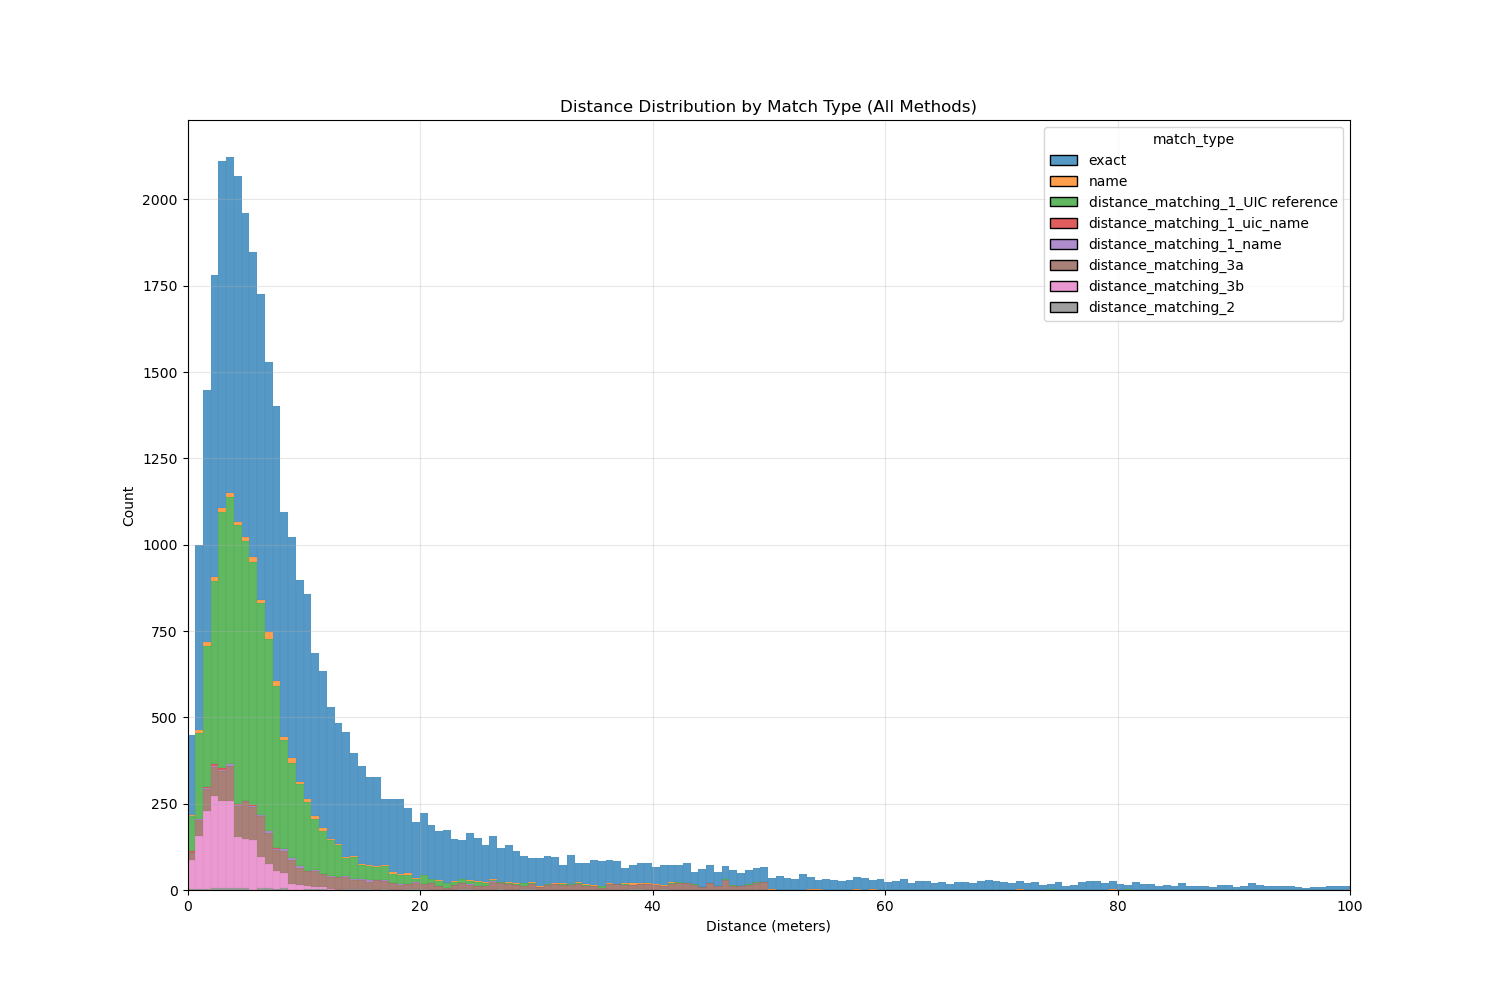
\includegraphics[width=\textwidth]{../figures/plots/distance_distribution_all.png}
    \caption[Distribution des distances par méthode]{Distributions des distances pour chaque méthode de correspondance}
    \label{fig:sample}
\end{figure}
Comme on peut le voir dans le graphique, à une coupe de 100 mètres, il y a une longue traîne de correspondances qu'il faut corriger. De plus, la médiane pour les correspondances exactes est très importante à 22 mètres.

Voici les statistiques :

\begin{itemize}
    \item \textbf{DISTANCE}
    \begin{itemize}
        \item Moyenne : 7,94 m
        \item Médiane : 5,37 m
    \end{itemize}
    
    \item \textbf{EXACT}
    \begin{itemize}
        \item Moyenne : 22,62 m
        \item Médiane : 9,40 m
    \end{itemize}
    
    \item \textbf{NAME}
    \begin{itemize}
        \item Moyenne : 36,64 m
        \item Médiane : 10,25 m
    \end{itemize}
\end{itemize}


